% !TeX root = ../Bachelorarbeit.tex
\chapter{Konzeption}
\section{Auswahl der Authentifizierungsverfahren}
Bei der Auswahl der Authentifizierungsverfahren musste vor allem berücksichtigt werden, inwiefern das Verfahren im Rahmen dieser Arbeit umsetzbar ist. Dies bezieht sich einerseits auf die Zeit, die es für die Implementation benötigt und andererseits auch auf die monetäre Machbarkeit. Es existieren für die Webauthentikation zum Beispiel ganz spezielle USB-Sticks von angesehenen Marken, die allerdings einige hunderte Euro kosten. Die Features die sie im Gegensatz zu einem ganz normalen USB-Stick (FIDO USB) liefern, beziehen sich dabei nur auf den Teil der Userverifikation. So besitzen einige USB-Sticks einen eingebauten Fingerabdrucksensor, ein Tastenfeld oder sogar zusätzliche Sicherheitssoftware auf den Massendatenträgern. Innerhalb dieser Arbeit sollte es allerdings um den Einsatz eines solchen Verfahrens für den Durchschnittsnutzer innerhalb von Unternehmen oder einen Casual Surfer gehen. Eine teure Anschaffung für die eigene Sicherheit erscheint dem Durchschnittsnutzer als nicht nötig.

Das Verfahren des Usernamen und des Passwortes wurde gewählt, weil es zum Verfassungszeitpunkt dieser Arbeit die Nutzer von Webseiten meist alleinig sichert. Die Loginverfahren größerer Dienste wie Microsoft Outlook, Google Mail und Facebook besitzen zwar schon seit Jahren die Möglichkeit der Authentifikation mit einem zweiten Faktor, doch das sind eher Ausnahmen. Ein Großteil der Internetpräsenzen ist sich entweder nicht der Risiken von Passwörtern für ihre Nutzer bewusst oder kann sich den Mehraufwand von neuen Verfahren nicht leisten. Gleichzeitig war es im Rahmen dieser Arbeit wichtig eine typische Implementation mit Username \& Passwort und ihren Scheinsicherheiten wie Hashes mit Salt und Pepper zu präsentieren. Es ist wichtig, den Ist-Zustand im heutigen Internet zu verstehen, um die Vorteile von neueren Methoden nachzuvollziehen.

Eine dieser neuen Methoden ist das zweite Verfahren. Nach dem Passwort ist das wohl der häufigste zweite Faktor den man findet. Apps wie der 'Google Authenticator' zählen mittlerweile als Synonym für das \ac{totp} - Verfahren wie es im RFC beschrieben ist. Dies liegt unteranderem auch daran, dass die App tatsächlich die recht strikten Vorgaben aus dem RFC befolgt und nur minimale Unterschiede dazu aufweist.
\newpage

An dieser Stelle stellte sich eher die Frage ob HOTP oder \ac{totp} in den Prototypen implementiert werden sollte. Es wurde sich für das \ac{totp} - Verfahren entschieden, da es zwar den Mehraufwand der Synchronisation zwischen Zeit des Gerätes und des Servers benötigt doch dafür die Sicherheit der begrenzten Zeit bietet wie bereits erläutert.

Das dritte Verfahren, die 'Web Authentication', ist wohl das Erforschungswürdigste der drei Verfahren. Sie ist von allen drei Verfahren am seltensten auf Internetseiten vertreten und da stellt sich nach einer Analyse des Mehrwertes dieses Verfahrens die Frage nach dem Grund dafür. Im Gegensatz zu den anderen beiden Authentifikationsmethoden wurde Dieses nicht für den Prototypen ausgewählt, weil es so weit verbreitet und bereits genutzt wird sondern genau im Gegenteil: Es wurde gewählt, um mögliche Gründe zu suchen weshalb das Verfahren der Webauthn heutzutage kein Standard darzustellen scheint. Es muss untersucht werden ob es starke Nachteile Gegenüber der anderen Verfahren bietet, denn im Ansatz scheint es alle Nachteile des Passwortes auszumerzen.
\newpage

\section{Authentifikation in drei Schichten}

\begin{center}
    \center
    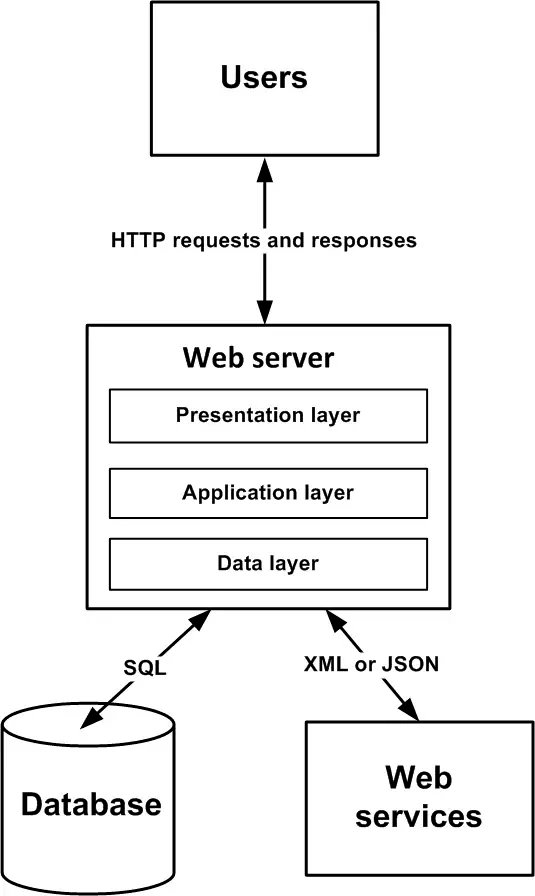
\includegraphics[width=10cm]{main-qimg-82af1fe49f85a31700d35570189a1fce.png}
\end{center} 

Das Ziel des Prototypen ist es, wie eingangs erwähnt, vorhandene Authentifizierungsverfahren abseits der klassischen UserID / Passwort Methode zu begutachten und dessen Schwächen aufzudecken. Daraus ergeben sich die typischen drei Komponenten von Drei-Tier-Client-Server Architekturen:

Ein Client, der Anfragen an die Applikation (das Backend bzw. den Server) sendet, welches die Daten dann in einer Datenbank mittels eines DBMS (Datenbankmanagementsystems) persistiert und verwaltet. Wie auch im Bild zur 3 Tier Architektur zu sehen, agiert der User auf dem Presentation Layer und stellt anfragen bzw. sendet JSON Objekte an den Server, der die entsprechenden Webservices liefert. Der Server speichert keine States, wodurch der Nutzer typischerweise mit jeder Anfrage alle benötigten Informationen liefern muss. Der Server liefert demnach lediglich die \ac{rest} Schnittstellen. Implementationsdetails und weitere Informationen zum Prototypen gibt es in folgenden Kapiteln.

\section{Kriterien für eine erfolgreiche Authentifikation}
Auch wenn die Frage: ``Ist eine gelungene Authentifikation auch eine erfolgreiche Authentifikation?'' eine philosophische zu sein scheint, ist sie dennoch nicht minder interessant. Es wurde bereits gezeigt, dass Nutzer nicht gewillt sind komplizierte und aufwendige Dinge zu tun, um sich selbst und ihre Daten im Internet zu schützen. Sofern also die Methodik der Webseite zu kompliziert ist, sucht der Nutzer sich Ausflüchte um die vorhandenden Verfahren so angenehm wie möglich zu machen, was wiederrum die Sicherheit ihrer Internetpräsenz gefährdet. Das Passwort besitzt zu viele Schwachstellen als das man eine Authentifikation damit als Erfolg verbuchen kann. Es scheint eher dem Zweck 'irgendeiner Schutzbariere zwischen fremder Person und Daten des Nutzers' zu dienen als wirklich zur 'Sicherheit'.

Überträgt man dieses Wissen auf die Kriterien dieser Arbeit ergeben sich folgende Anforderungen:

\begin{itemize} 
\item \textbf{Nutzerfreundlichkeit}

Angefangen der Nutzerfreundlichkeit, einem der wichtigsten Kriterien für die Authentifikation, welches in direktem Bezug zur Sicherheit steht [A24] [A25] [A26]. Der Prototyp soll eine einfache Authentifikation ermöglichen. Keine häufigen Weiterleitungen, keine Popups, keine langen Ladezeiten und vorallem zwecks Authentifizierung: Keine sinnfreie Aneinanderschaltung von verschiedenen Sicherheitsfaktoren.
\newpage

Ein Beispiel für solch eine Praktik wäre, dass nach der Bestätigung des Einloggvorgangs durch Fingerabdruck zusätzlich eine PIN und in folge dessen ein Sicherheitsschlüssel (mit zusätzlich benötigtem PIN) verlangt wird, obwohl nach dem ersten Schritt des Fingerabdrucks bereits die Authentizität des Users festgestellt wurde. So muss der Prototyp am Besten aus nur einem Faktor der Sicherheit bestehen und dem Nutzer die Auswahl zur Selbstentscheidung über die verschiedenen Möglichkeiten bieten, so wie es bei der adaptiven MFA (anhand von selektierten Faktoren) auch der Fall ist. Im konkreten Fall des Prototyps soll es demnach auch reichen nur einen der registrierten Geräte für die Web Authentication zu nutzen, so kann der User bequem die PIN zur Authentifizierung nutzen. Falls der Rechner dies nicht unterstützt, kann der User zum Sicherheitsschlüssel greifen oder das Smartphone für das \ac{totp} - Verfahren verwenden.

\item \textbf{Sicherheit}

Der Prototyp möglichst unnötige Metadaten vermeiden. Dazu sollen meist die selben Statuscodes und nur allgemeine Fehlermeldungen bei nicht erfolgreicher Authentifikation zurückgegeben werden. So ist die Nachricht ``Das Passwort ist inkorrekt.'' als obsoluter Fehler zu betrachten, da ein Angreifer nun die Möglichkeit hat, durch einen Bruteforce - Angriff auf das Loginformular das richtige Passwort zu erraten. Diese Nachricht würde nämlich implizieren, dass ein Nutzer mit eingegebenem Nutzernamen in der Datenbank vorhanden ist, doch das Passwort nicht stimmt. Stattdessen werden allgemeine Responsemessages gegeben wie ``Der Benutzername oder das Passwort sind falsch.'', um dem Angreifer keinerlei Metadaten auszuhändigen.

Gleichzeitig muss die Verbindung zum Backend, auch im Prototyp, durch ein eigenes SSL - Zertifikat gesichert sein. \ac{mitm} - Angriffe sind, wie bereits erläutert, nicht immer verhinderbar. In unserem Falle sind wir selbst der Aussteller des Zertifikats und vertrauen uns selbst. Ein User kann (und wird) allerdings nicht die Vertrauenswürdigkeit seines Zertifikates erfragen.

Wenn man die drei Verfahren nach ihrer Sicherheit ordnet, käme an hinterster Stelle wohl das Passwort. Wieso wurde bereits erläutert. Darauf würde das \ac{totp} - Verfahren kommen, das so lange sicher ist wie das Gerät welches die \ac{totp} - Codes erfragt sicher ist.
\newpage

Hat man seinen QR-Code also im Google Authenticator eingescannt und lässt sein Smartphone ungesichert an einem öffentlichen Ort liegen, sind die aufzubringenden Ressourcen für den Angreifer recht gering. Er kann sich das Smartphone nehmen, die App öffnen und den Code auf der Webseite eingeben. Je nach Betriebssystem können sich weitere Angriffsmöglichkeiten ergeben. So ist es auf Smartphones mit dem Betriebssystem IOS relativ schwierig an appeigene Daten zu gelangen, da jede App in ihrer eigenen Sandbox mit ganz speziellen Rechten geöffnet wird. Auf Android-Smartphones sieht dies bereits anders aus. Dort gibt es einen geteilten Zwischenspeicher, welches den Zugriff auf Daten anderer Apps begünstigt. So könnte man einen Screenshot machen und diese per Mail an den Angreifer weiterleiten. Andere bekannte Angriffe auf \ac{totp} - Verfahren sind soweit nicht bekannt. Das sicherste Verfahren (aus den ausgewählten im Rahmen dieser Arbeit) ist die Webauthentikation. Sie bietet wenig Angriffsfläche, dadurch das die privaten Schlüssel an einem sicheren Ort im Betriebssystem persistiert werden und man nicht so leicht an diese kommt. Der öffentliche Schlüssel besitzt keinen Wert und wird vom Authenticator generiert. Dadurch ist kein Zutuen des Nutzers erforderlich wie bei einem Passwort. Dieses Verfahren ist auch relativ sicher gegen \ac{mitm} - Angriffe, da ein Angreifer maximal die Challenge des Servers abfangen kann, um sein eigenes Gerät für einen Nutzer zu registrieren. Dies erfordert allerdings entweder eine komplette Kontrolle über den Rechner (Remote Access Control) oder phsysischen Zugriff auf den Rechner durch den Angreifer.

\item \textbf{Datenschutz}

Die Forschungsfrage dieser Arbeit ist überhaupt erst entstanden, durch einen Datenschutzvorfall bei Firmen. Auch wenn der Datenschutz bis jetzt nicht viel Erwähnung fand, ist er neben der Sicherheit und der Nutzerfreundlichkeit kein minderes Kriterium für eine erfolgreiche Authentifikation. Zum Schutz der Daten gehört zum Beispiel, SQL - Injektionen durch das Benutzen von 'Prepared SQL Statements' zu verhindern. Dies bedeutet, dass Userdaten an keiner Stelle unformatiert in ein SQL Schnipsel eingebaut werden. Gleichzeitig muss sichergestellt werden, dass der Prototyp bei erfolgreichem Login keinerlei Metadaten über den Nutzer preisgibt. So wäre es ein Datenschutz-Problem wenn bei der Authentifikation über Webauthn zusätzliche Daten wie die E-Mail des Nutzers, sein Passwort und die Zeit der Erstellung des Accounts mitgesendet werden. Das Prinzip sollte stets lauten: So wenig Daten wie nötig. Das Recht auf informetionelle Selbstbestimmung ist hier insofern gewährleistet, dass der User selbst entscheiden kann, ob er einen \ac{totp} registriert oder welches Gerät er für die Webauthn nimmt.
\newpage

Ein großer Vorteil neuerer Verfahren ist, dass hinter einer \ac{totp} oder Webauthn - Geräteregistration keinerlei persönliche Daten stehen. Selbst wenn Angreifer also den gesamten Registrationsprozess auf dem Gerät mitschneiden, können sie daraus keine verwertbaren Metadaten für zukünftige Angriffe erlangen.
\end{itemize}
